\documentclass{homework}
\usepackage[utf8]{inputenc}
\usepackage{graphicx}
\usepackage{hyperref}
\hypersetup{
    colorlinks=true,
    linkcolor=blue,
    filecolor=magenta,      
    urlcolor=cyan,
    pdftitle={Overleaf Example},
    pdfpagemode=FullScreen,
    }
\def\one{\mbox{1\hspace{-4.25pt}\fontsize{12}{14.4}\selectfont\textrm{1}}} % 11pt    

\title{EP 2 - MAP 2212}
\author{Nicholas Gialluca Domene - N USP 8543417}

\begin{document}

\maketitle

\section{2nd Programming Exercise}

- Find out how to use, in your computational environment, library functions to generate random variables with Uniform, Beta, Gamma and Weibull distributions.

- Implement the four variants of Monte Carlo integration we studied to integrate the function $f(x) = e^{-ax}cos(bx)$ in $[0, 1]$, where $a = 0.RG$, $b = 0.CPF$, and RG and CPF stand for digits of your official IDs.

- Choose parameters for each sampling distribution by visual inspection or any other method you like (adapt domain?). Choose a polynomial function for control variate. Choose $n$ to get a relative error $\frac{|\hat\gamma - \gamma |}{\gamma} < 0.0005$ (without knowing $\gamma$!)

- Write well documented source codes and a nice LaTeX report explaining everything you did and the choices you made. Deliver your zip file at e-disciplinas by ??/??/202?

- Discuss your ideads, but do your own work. Good luck!

\section{Solution}

\subsection {Definitions and pre-requisites}

\subsubsection{}
 Since I am using Python for the Programming Exercise solution, these are the methods for generating a random variable in each distribution:

-> Uniform distribution between interval a and b given $a, b \in \R, a \leq b$

\begin{lstlisting}
import numpy as np
random_number = np.random.uniform(low=a, high=b)
\end{lstlisting}

-> Beta distribution with parameters $a, b \in \R$

\begin{lstlisting}
import numpy as np
random_number = np.random.beta(a=a_beta, b=b_beta)
\end{lstlisting}

-> Gamma distribution with parameters $a, b \in \R$

\begin{lstlisting}
import numpy as np
random_number = np.random.gamma(a, b)
\end{lstlisting}

-> Weibull distribution with parameter $a \in \R$

\begin{lstlisting}
import numpy as np
random_number = np.random.weibull(a)
\end{lstlisting}

\subsubsection{}
Defining f(x) as follows and defining f(x) domain as $x \in [0, 1]$:

\begin{lstlisting}
import math
def f(x):
    rg  = 0.384850546
	cpf = 0.45361387819
	return math.exp(-rg*x)*math.cos(cpf*x)
\end{lstlisting}

\begin{figure}[htp]
    \centering
    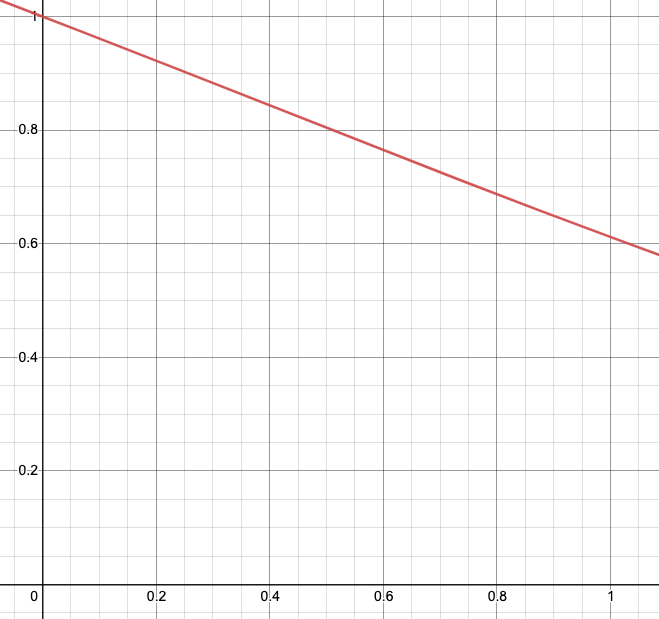
\includegraphics[width=10cm]{Screen Shot 2021-05-16 at 17.28.17}
    \caption{Generated using https://www.desmos.com/calculator}
\end{figure}

Since $\max f(x) = 1$ and $f(x) > 0, \forall x \in [0, 1]$, we see that $f(x)$ is inside the unit square $[0, 1]x[0, 1]$ and therefore $\int\limits_0^1 f(x) dx\leq 1$

\subsubsection{}
For reference, I ran the desired output on Wolfram Alpha and got:
\begin{equation}
    \int_0^1 f(x)dx = 0.804542
\end{equation}
As can be verified in the link  \url{https://www.wolframalpha.com/input/?i=integrate+exp%28-0.384850546x%29cos%280.45361387819x%29+from+0+to+1}

\subsection {Four variants implementation} 

As asked in the video, in this section I will determine an $n \in \R$ such that for each variant implementation the relative error (defined as $\frac{|\hat\gamma - \gamma |}{\gamma}$) will be $< 0.0005$.
The overall strategy will be: treat each implementation as an experiment design that using the defined steps and also the proposed n, the obtained experiment result will give an estimate for the true value of $\int_0^1 f(x)dx$ and a confidence interval of less than 0.0005\% the estimated value with 95\% confidence

For \bold{Crude Monte Carlo}, \bold{Importance Sampling} and \bold{Control Variates} methods, since there is not way to determine $n$ without running experiments and verifying the obtained variance, I defined a function \verb|run_experiment_increasing_n| that runs each implementation with an increasing given $n$ until it reaches a $n$ that returns an estimate with a relative error smaller than the given threshold of $0.0005$. At each retry, $n$ will double meaning that n will be $2^i$ in the i-th retry.

\begin{lstlisting}
def run_experiment_increasing_n(variant_implementation_function):
	is_error_below_threshold = False
	n = 1
	while is_error_below_threshold == False:
		n *= 2
		gamma_hat, is_error_below_threshold = variant_implementation_function(n)

	return gamma_hat, n
\end{lstlisting}

\subsubsection{Crude Monte Carlo}

Given the definitions presented in the Youtube video:

\begin{equation}
    \gamma = \int_a^b f(x)dx, \;\;\;\;\;\; x_i \sim U_{[a, b]}, \;\;\;\;\;\; \hat \gamma_c = \frac{1}{n}\sum_{i=1}^n f(x_i);
\end{equation}

\begin{equation}
    E(\hat \gamma_c) = \gamma, \;\;\;\;\;\; \sigma_c^2 = \frac{1}{n}\int_a^b[f(x) - \gamma]^2dx;
\end{equation}

For the implementation, I chose to define a function called \verb|crude| that will receive a parameter $n$ that is the number of points to be generated as to estimate the desired value (integral of f(x) from 0 to 1) and returns the gamma hat ($\hat \gamma$) that is the estimate for the desired output and a boolean variable \verb|is_error_below_threshold| that is \verb|True| if the obtained relative error is below the threshold and \verb|False| if not. The relative error is defined as the confidence interval with 95\% confidence defined as:

\begin{equation}
e = \frac{1.65*\sqrt{\frac{Var(\hat \gamma)}{n}}}{\hat \gamma}
\end{equation}

\begin{lstlisting}
def crude(n):
	#int -> float (gamma hat), boolean (is relative error below 0.0005)
	'''
	Receives an integer n that will be used to generate n points
	and generate the value of gamma hat, estimation for the integral
	of f(x) in the interval [0, 1], and its variance
	'''
	list_f_x = []
	gamma_hat = 0
	for i in range(n):
		x = np.random.uniform(low=0, high=1)
		f_x = f(x)
		list_f_x.append(f_x)
		gamma_hat += f_x/n

	variance_gamma_hat = np.var(list_f_x)

	standard_error = math.sqrt(variance_gamma_hat/n)
	is_error_below_threshold = True if (1.65*standard_error)/gamma_hat < 0.0005 else False

	return gamma_hat, is_error_below_threshold
\end{lstlisting}

Running \verb|run_experiment_increasing_n| for Crude implementation, it returns that $n = 262144$ is sufficient to return the desired estimate with a smaller than $0.0005$ relative error.

Execution output example:
\begin{lstlisting}
Crude Implementation
Gamma hat:  0.8047024676332211
N:          262144
Time taken: 0:00:00.740980
\end{lstlisting}







\subsubsection{Hit or Miss Monte Carlo}

Given the definitions presented in the Youtube video:

\begin{equation}
    h(x, y) = \one(y \leq f(x)); \;\;\;\;\;\; \gamma = \int_0^1 \int_0^1 h(x, y)dxdy;
\end{equation}

\begin{equation}
    \hat \gamma_h = \frac{1}{n}\sum_{i = 1}^n h(x_i, y_i); \;\;\;\;\;\; \sigma_h^2 = \frac{\gamma(1 - \gamma}{n};
\end{equation}


\begin{equation}
    \sigma_h^2 - \sigma_c^2 = \frac{1}{n}f(x)(1 - f(x))dx > 0
\end{equation}

Since $f(x) \in [0, 1] \forall x \in [0, 1]$, $\int_0^1 f(x)$ can be interpreted as the probability of any given point $(x_i, y_i) \forall (x_i, y_i) \in \R^2, x_i, y_i \in [0, 1]$ falling below the curve $f(x)$. Therefore, this can be interpreted as an estimation of a probability of event p happening and the Binomial distribution is a suitable fit.

By algebraic manipulation and working from the Normal approximation of the Binomial distribution, our $n$ can be found as follows:
\begin{equation}
Z_{score} = \frac{mdd}{\sqrt\frac{\sigma^2}{n}}
\end{equation}
\begin{equation}
Z_{score}*\frac{\sqrt{\sigma^2}}{\sqrt{n}} = mdd
\end{equation}
\begin{equation}
\frac{Z_{score}*\sqrt{\sigma^2}}{mdd} =\sqrt{n}
\end{equation}
\begin{equation}
n = \frac{Z_{score}^2 * \sigma^2}{mdd^2}
\end{equation}

where $mdd$ is the Minimal Detectable Difference, which in this case is 0.0005\%, meaning that in the worst possible case it will be $0.0005$ (if $\int_0^1 f(x)dx = 1$). So working from worst case scenarios:


\begin{equation}
    mdd = 0.0005; \;\;\;\;\;\; Z_{score} = 1.65; \;\;\;\;\;\; \sigma^2 = 0.25
\end{equation}

\begin{equation}
    n = \frac{1.65^2 * 0.25}{0.0005^2} = 2722500
\end{equation}

For the implementation, I chose to define a function called \verb|hit_or_miss| that will receive a parameter $n$ that is the number of points to be generated as to estimate the desired value (integral of f(x) from 0 to 1) and returns the gamma hat ($\hat \gamma$) that is the estimate for the desired output and a boolean variable \verb|is_error_below_threshold| that is \verb|True| if the obtained relative error is below the threshold and \verb|False| if not.

\begin{lstlisting}
import math
import numpy as np

def hit_or_miss(n):
	#int -> float (gamma hat), boolean (is relative error below 0.0005)
	'''
	Receives an integer n that will be used to generate n points
	and generate the value of gamma hat, estimation for the integral
	of f(x) in the interval [0, 1], and its variance
	'''
	gamma_hat = 0
	for i in range(n):
		x = np.random.uniform(low=0, high=1)
		y = np.random.uniform(low=0, high=1)
		f_x = f(x)
		if y <= f_x:
			gamma_hat += 1

	gamma_hat = gamma_hat/n
	variance_gamma_hat = gamma_hat*(1 - gamma_hat)

	standard_error = math.sqrt(variance_gamma_hat/n)
	is_error_below_threshold = True if (1.65*standard_error)/gamma_hat < 0.0005 else False

	return gamma_hat, is_error_below_threshold
	
print("Hit or Miss Implementation")
t0 = datetime.datetime.now()
gamma_hat, is_error_below_threshold = hit_or_miss(2722500)
t1 = datetime.datetime.now()
print("Gamma hat: ", gamma_hat)
print("Is error below threshold: ", is_error_below_threshold)
print("Time taken: ", t1-t0)
print()
\end{lstlisting}


Execution output example:
\begin{lstlisting}
Hit or Miss Implementation
Gamma hat:  0.8044080808080808
Is error below threshold:  True
Time taken:  0:00:05.026397
\end{lstlisting}









\subsubsection{Importance Sampling}

Given the definitions presented in the Youtube video:

\begin{equation}
    \gamma = \int_a^b f(x)dx = \int \frac{f(x)}{g(x)}g(x)dx; \;\;\;\;\;\; x_i \sim g(x);
\end{equation}

\begin{equation}
    \hat \gamma_s = \frac{1}{n}\sum_{i=1}^n \frac{f(x_i)}{g(x_i)}; \;\;\;\;\;\; \sigma_s^2 = \frac{1}{n}\int \left(\frac{f(x)}{g(x)} - \gamma\right)^2 g(x)dx
\end{equation}

For the implementation, I chose to define a function called \verb|importance_sampling| that will receive a parameter $n$ that is the number of points to be generated as to estimate the desired value (integral of f(x) from 0 to 1) and returns the gamma hat ($\hat \gamma$) that is the estimate for the desired output and a boolean variable \verb|is_error_below_threshold| that is \verb|True| if the obtained relative error is below the threshold and \verb|False| if not. The relative error is defined as the confidence interval with 95\% confidence defined as:

\begin{equation}
e = \frac{1.65*\sqrt{\frac{Var(\hat \gamma)}{n}}}{\hat \gamma}
\end{equation}

From try-and-error inspection, I have chosen the approximating distribution function Beta with parameters $\alpha = 1$ and $\beta = 1$, meaning that each random returning point will follow $X_i \sim \beta(1, 1)$.


Using the immediacy from the definition of variance stating that $\sigma^2(x) = E(x^2) - E^2(x)$, the function definition in Python is as:

\begin{lstlisting}
import math
import numpy as np
from scipy.stats import beta

def beta_density(x, alpha, beta):
	beta_hat = math.gamma(alpha)*math.gamma(beta)/math.gamma(alpha+beta)
	return (x**(alpha - 1)*(1 - x)**(beta-1))/beta_hat
	
def importance_sampling(n):
	#int -> float (gamma hat), boolean (is relative error below 0.0005)
	'''
	Receives an integer n that will be used to generate n points
	and generate the value of gamma hat, estimation for the integral
	of f(x) in the interval [0, 1], and its variance
	'''
	a_beta, b_beta = 1, 1 #determined visually
	gamma_hat = 0
	gamma_hat2 = 0
	for i in range(n):
		x = np.random.beta(a=a_beta, b=b_beta)
		f_x = f(x)
		f_x2 = f(x**2)
		g_x = beta_density(x, a_beta, b_beta)
		g_x2 = beta_density(x**2, a_beta, b_beta)
		gamma_hat += (f_x/g_x)/n
		gamma_hat2 += (f_x2/g_x2)/n

	variance_gamma_hat = gamma_hat2 - gamma_hat**2

	standard_error = math.sqrt(variance_gamma_hat/n)
	is_error_below_threshold = True if (1.65*standard_error)/gamma_hat < 0.0005 else False

	return gamma_hat, is_error_below_threshold

\end{lstlisting}


Execution output example:
\begin{lstlisting}

Importance Sampling Implementation
Gamma hat:  0.8044942478962475
N:          4194304
Time taken: 0:00:25.117877
\end{lstlisting}









\subsubsection{Control Variates}

For this implementation, I chose the polynomial function $\varphi(x) = g(x) = 1 - \frac{2}{5}x$ as it is simpler to integrate and it approximates relatively well f(x) as it can be verified by the following graph:

\begin{figure}[htp]
    \centering
    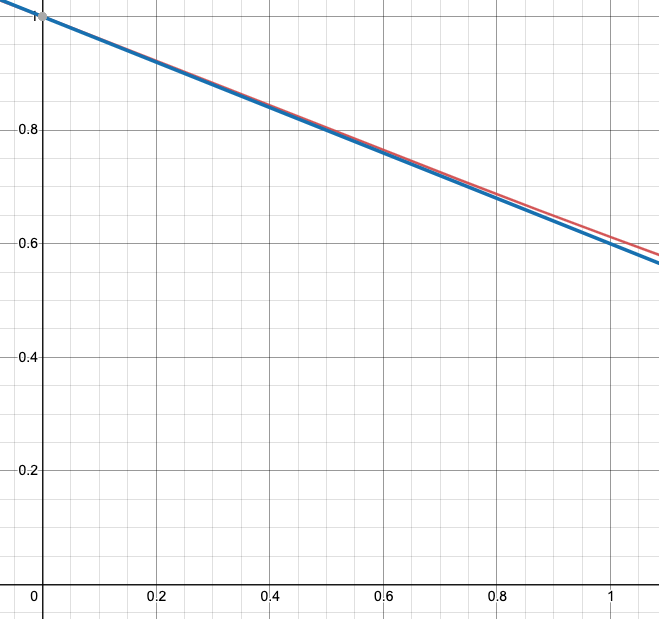
\includegraphics[width=10cm]{Screen Shot 2021-05-16 at 17.28.37}
    \caption{Generated using https://www.desmos.com/calculator \n Red line is f(x), blue line is g(x)}
\end{figure}

\begin{equation}
    \int_0^1 g(x) dx= \int_0^1 1 - \frac{2}{5}x dx= [x - \frac{2x^2}{10}]|_0^1 = 1 - \frac{1}{5} = \frac{4}{5}
\end{equation}

The following definitions were given for estimating $\hat \gamma$:

Let $\varphi(x)$ be a control variate

\begin{equation}
    \gamma = \int [f(x) - \varphi(x) + \varphi(x)]dx, \gamma' = \int \varphi(x)dx
\end{equation}
\begin{equation}
    \hat \gamma = \frac{1}{n}\sum_1^n [f(x_i] - \varphi(x_i) + \gamma']
\end{equation}
\begin{equation}
    Var(\hat\gamma) = \frac{1}{n} [ \sigma^2(f(x)) + \sigma^2(\varphi(x)) - 2 \rho(f(x), \varphi(x))\cdot\sigma(f(x))\cdot\sigma(\varphi(x))]
\end{equation}
Where $\rho$ is assumed to be the Pearson correlation between the variables, $\sigma$ is assumed to be the standard deviation of each variable and $\sigma^2$ is assumed to be the variance of each variable.

I used $\varphi(x) = g(x) = 1 - \frac{2}{5}x$, so $\gamma' = \int g(x)dx = \frac{4}{5}$, therefore

\begin{equation}
    \hat \gamma = \frac{1}{n}\sum_1^n [f(x_i] - \varphi(x_i) + \frac{4}{5}]
\end{equation}

For the implementation, I chose to define a function called \verb|control_variate| that will receive a parameter $n$ that is the number of points to be generated as to estimate the desired value (integral of f(x) from 0 to 1) and returns the gamma hat ($\hat \gamma$) that is the estimate for the desired output and a boolean variable \verb|is_error_below_threshold| that is \verb|True| if the obtained relative error is below the threshold and \verb|False| if not. The relative error is defined as the confidence interval with 95\% confidence defined as:

\begin{equation}
e = \frac{1.65*\sqrt{\frac{Var(\hat \gamma)}{n}}}{\hat \gamma}
\end{equation}


\begin{lstlisting}
import math
import numpy as np
from scipy.stats.stats import pearsonr

def control_variate(n):
	#int -> float (gamma hat), boolean (is relative error below 0.0005)
	'''
	Receives an integer n that will be used to generate n points
	and generate the value of gamma hat, estimation for the integral
	of f(x) in the interval [0, 1], and its variance
	'''
	def g(x):
		return 1 - (2/5)*x

	#store lists to calculate correlation and variance
	list_f_x  = []
	list_g_x  = []
	gamma_hat = 0
	for i in range(n):
		x   = np.random.uniform(low=0, high=1)
		f_x = f(x)
		g_x = g(x)
		list_f_x.append(f_x)
		list_g_x.append(g_x)
		gamma_hat += (f_x - g_x + 4/5)/n

	'''
	pearsonr returns two values: Pearson’s correlation coefficient
	and the 2-tailed p-value, according to the documentation
	https://docs.scipy.org/doc/scipy/reference/generated/scipy.stats.pearsonr.html
	'''
	rho = pearsonr(list_f_x, list_g_x)[0]

	var_f_x = np.var(list_f_x)
	stddev_f_x = math.sqrt(var_f_x)
	var_g_x = np.var(list_g_x)
	stddev_g_x = math.sqrt(var_g_x)

	variance_gamma_hat = (1/n)*(
		var_f_x + var_g_x - 2*rho*stddev_f_x*stddev_g_x
		)

	standard_error = (math.sqrt(variance_gamma_hat)/math.sqrt(n))
	is_error_below_threshold = True if (1.65*standard_error)/gamma_hat < 0.0005 else False

	return gamma_hat, is_error_below_threshold
\end{lstlisting}

Execution output example:
\begin{lstlisting}
Control Variate Implementation
Gamma hat:  0.8043731436065886
N:          16
Time taken: 0:00:00.112826
\end{lstlisting}



\end{document}
